\section{Testbench Architecture}

The testbench of the MCE uses a grey box view of the design.
Meaning, that the current state of the DUT is not only determined by the information gathered at the interfaces, but also by internal signals.
On the one hand this has the downside, that the testbench is dependent upon the internal structure of the design.
So internal changes in the design can require adjustments of the testbench, which typically should be avoided.
On the other hand this makes it easier to check the behavior of the DUT.
Since the interfaces of the design provide only limited information about the current state of the design itself, the grey box view is necessary to collect enough coverage data to verify the engine.\\ 
Structural the testbench of the MCE consists of two interface UVCs, a module UVC and a virtual sequence driver (figure~\ref{fig:mce_tb}).\\
The interface UVCs are used to handle the interfaces of the engine.
Thereby, the CSR UVC is responsible for the memory interface.
The other interfaces are grouped together in the \emph{ProgramFlow} UVC and a virtual sequence driver is used to coordinate the interaction between the individual interfaces.\\
The transactions produced by the interface UVCs are sent to the module UVC to check the behavior of the MCE across the different interfaces.
The module UVC additionally collects data of the internal state of the design.



\begin{figure}[htb]
 \centering
 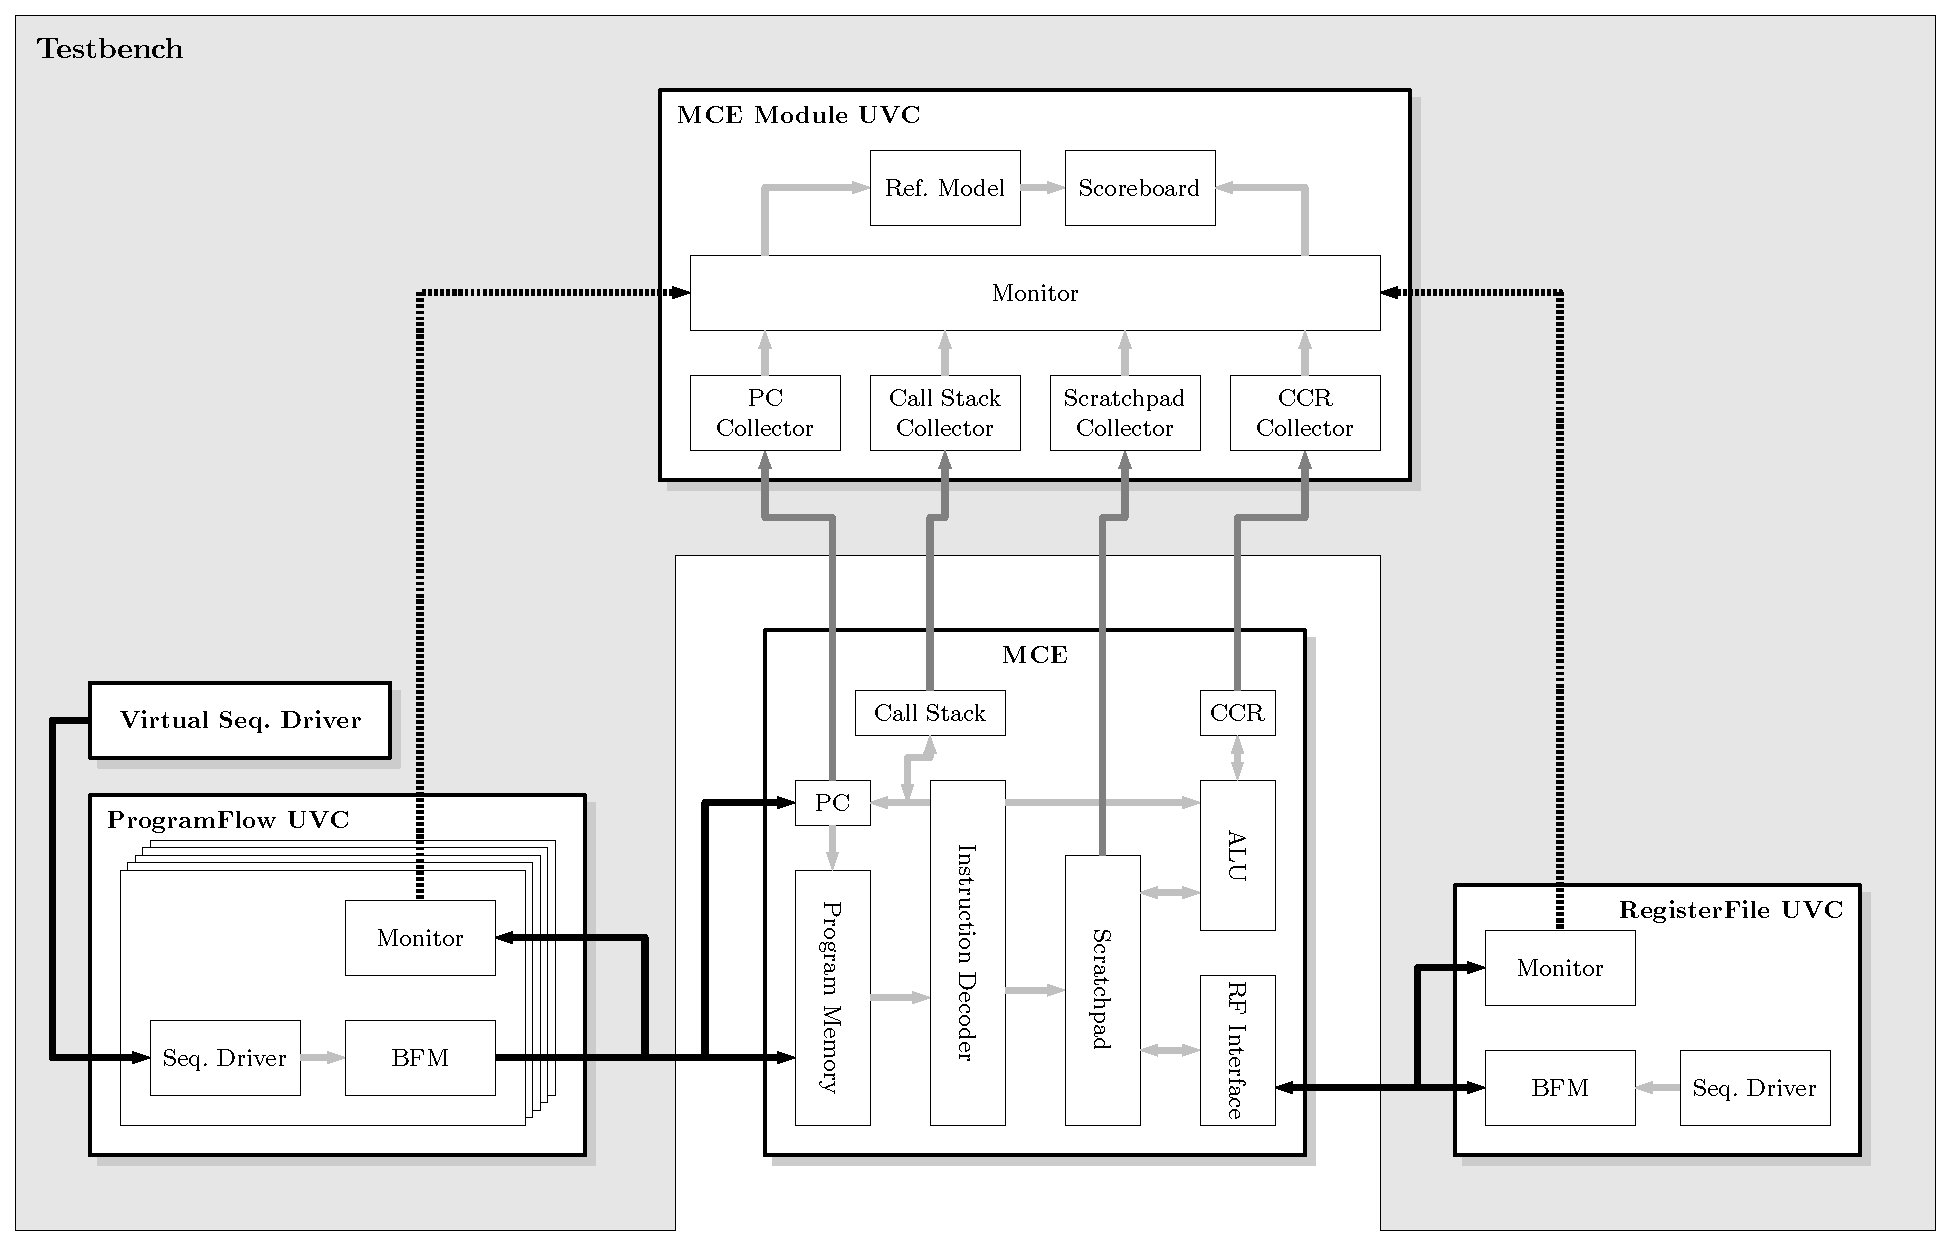
\includegraphics[width=1.0\textwidth,angle=0]{images/mce_tb}
 \caption{MCE Testbench}
\label{fig:mce_tb}
\end{figure}

\subsection{ProgramFlow Interface UVC}

The ProgramFlow interface UVC groups multiple interfaces of the MCE. 
It handles the instruction memory, external condition code bits, call stack overflow, start and done interfaces.
Thereby each interface has its own agent.
These agents are described in the following sections.

\subsubsection{Instruction Memory Agent}

The instruction memory agent is responsible for driving and monitoring the instruction memory interface of the MCE.
It can either be active or passive.
When the agent is active, it uses a sequence driver to send transactions to the BFM.
Thereby a transaction consists of a 32~bit instruction and a 12~bit address.
The instruction is thereby a separate sequence item, consisting of the individual fields of the instruction.
Within that, when-subtyping is used to group the fields for each type of instruction identified by its opcode.
The BFM then writes the instruction into the desired address of the instruction memory by applying both field to their corresponding signals of the interface.
In addition \emph{write\_en} is asserted for a single clock cycle to indicate that the assigned address and data are valid.\\
Independent of weather the agent is active or passive. The monitor collects data from the interface. It creates a sequence item and sends it via its TLM port to
the module UVC. An item is created every clock cycle the \emph{write\_en} is asserted. 
In addition, coverage is collected for the interface, whenever a sequence item is created.


\subsubsection{External Condition Code Bits Agent}

Similar to the instruction memory agent, the external condition code bits agent consists of a sequence driver and BFM to drive signals into the DUT and a
monitor to collect data from the connected interface.
When the sequence driver sends a transaction to the BFM, its value is directly assigned to the \emph{ext\_cc\_bits} signal of the interface.
Comparable to the CCR, the 16 bit signal is split into 4 4~bit groups. Thus, a transaction consists of a 4~bit data field and a 4~bit index, which specifies the
group of bits. So always 4 bits are set at once.\\
The monitor creates always a sequence item, when a bit is changed within a 4~bit group. 
So in a single clock cycle up to 4 transactions can be created and send to the module UVC.
In addition, coverage is collected for the interface, whenever a sequence item is created.

\subsubsection{Call Stack Overflow Agent}

Since the call stack overflow interface, does not contain any signals, that are inputs to the DUT, the corresponding is a purely passive one.
This means, that it only contains a monitor and no sequence driver or BFM.
It creates a transaction, whenever the \emph{call\_stack\_overflow} signal rises and sends it to the module UVC and virtual sequence driver.
In addition, coverage is collected for the interface, whenever a sequence item is created.

\subsubsection{Start Agent}

In contrast to the call stack overflow agent, the start agent can again be active or passive.
When the sequence driver sends a transaction to the BFM, it is used to drive the start interface.
Thereby, a transaction consists of the start address, which is then assigned to the corresponding signal of the interface.
In addition, the \emph{start} signal is asserted for a single clock cycle to indicate, that the value of \emph{start\_address} is valid.\\
The monitor of the start agent creates a sequence item, whenever the \emph{start} signal of the interface is asserted.
The item consists of the value available at the \emph{start\_address} signal and is send to the module UVC and virtual sequence driver.
In addition, coverage is collected for the interface, whenever a sequence item is created.

\subsubsection{Done Agent}

Similar to the call stack overflow interface, the done interface does not contain any inputs to the DUT.
Therefore, it is also a pure passive component, containing only a monitor.
It creates a transaction, whenever the \emph{done} signal rises and sends it to the module UVC and virtual sequence driver.
In addition, coverage is collected for the interface, whenever a sequence item is created.

\subsection{CSR Interface UVC}

The external memory interface is handled in the CSR interface UVC.
Its monitor samples the individual signals of the interface and creates a sequence item for each CSR access with the collected data.
This item consists of the direction of the operation (read or write), the address within the CSR, the data read from or written to the CSR and a flag
indicating, weather the address was valid or not. 
It is then sent to the module UVC via a TLM port.\\
When the MCE starts a transaction, the UVC has to respond to this request.
Therefore, the UVC contains a slave agent.
So if the monitor notices, that a transaction has been started, it emits an event, causing the sequence driver to generate the response.
Since a memory access can take multiple clock cycles to complete, first a random number of up to 10 clock cycles is waited.
After that the UVC sends the access complete signal and additionally random data is returned for a read transaction.
Furthermore there is a chance, that the transaction is completed indicating an invalid address in addition to the access complete signal.
In addition, the monitor performs checks to ensure, that transaction on the interface are always started and completed correctly and coverage is collected.

\subsection{MCE Module UVC}

The module UVC of the MCE has knowledge of the desired behavior of the DUT.
It uses a reference model to predicts the behavior of the engine for a given set of stimuli.
In the scoreboard the predicted results are then matched against the data received from the interface UVCs and its own collectors.
With this flow the behavior of the engine is automatically checked.
This self-checking is crucial to a coverage-driven verification flow, since the stimuli generation is also automated.
The structure of the module UVC is shown in figure~\ref{fig:module_uvc}.

\begin{figure}[htb]
 \centering
 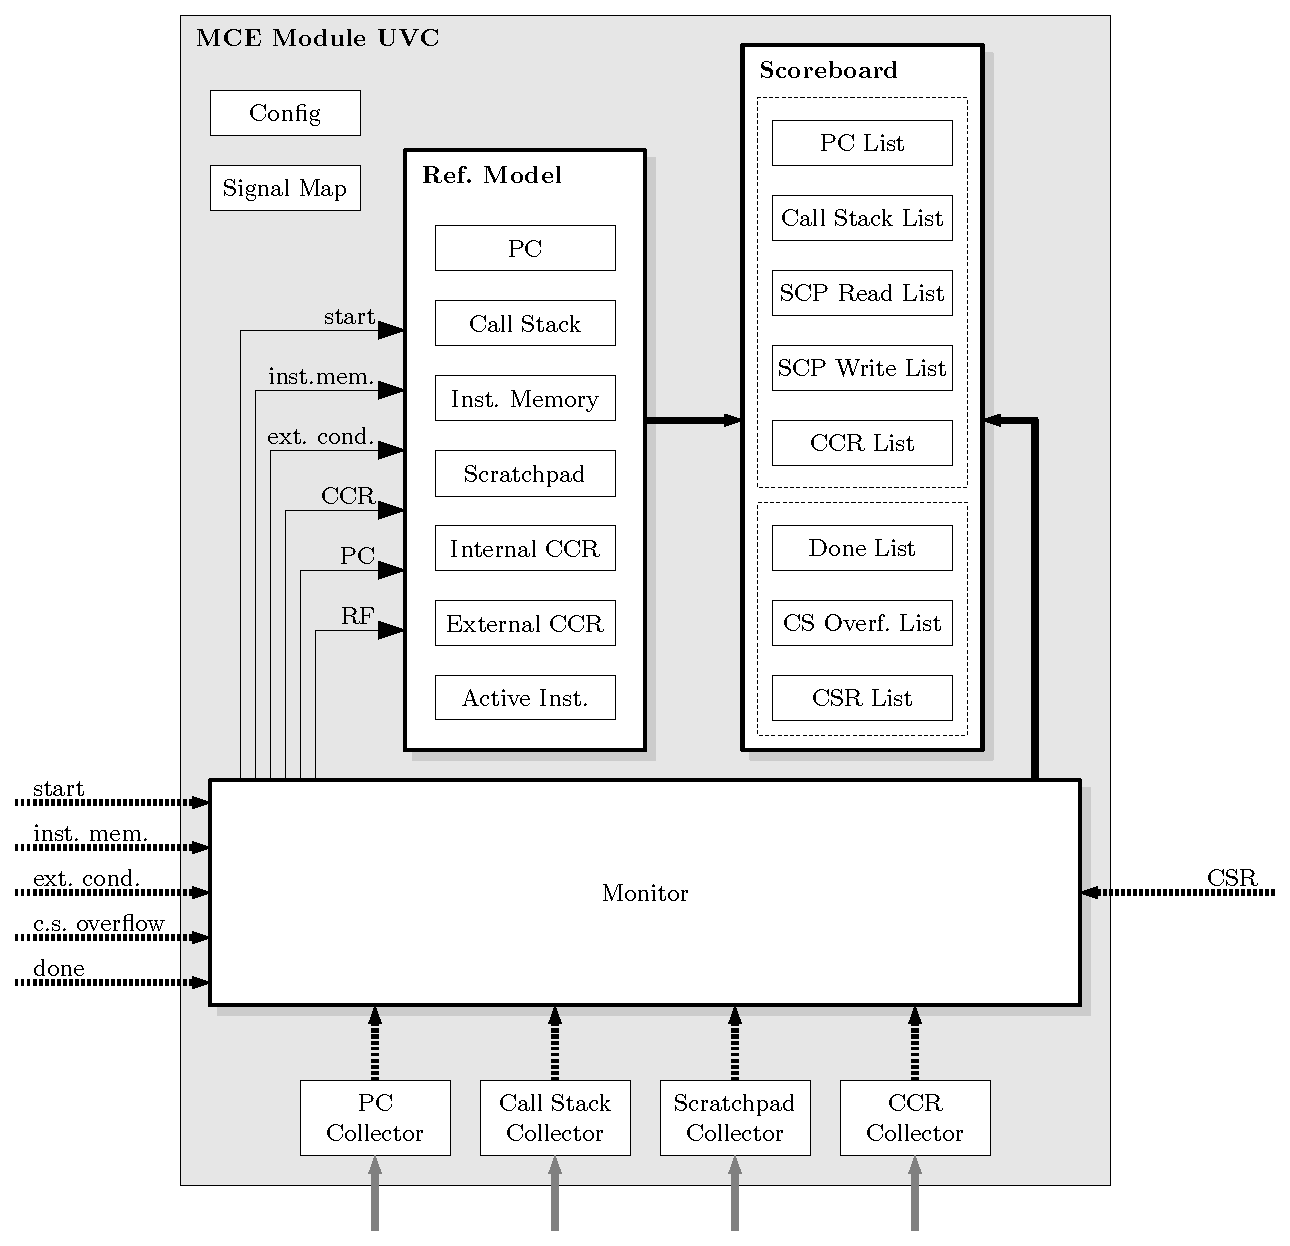
\includegraphics[width=1.0\textwidth,angle=0]{images/mce_module_uvc}
 %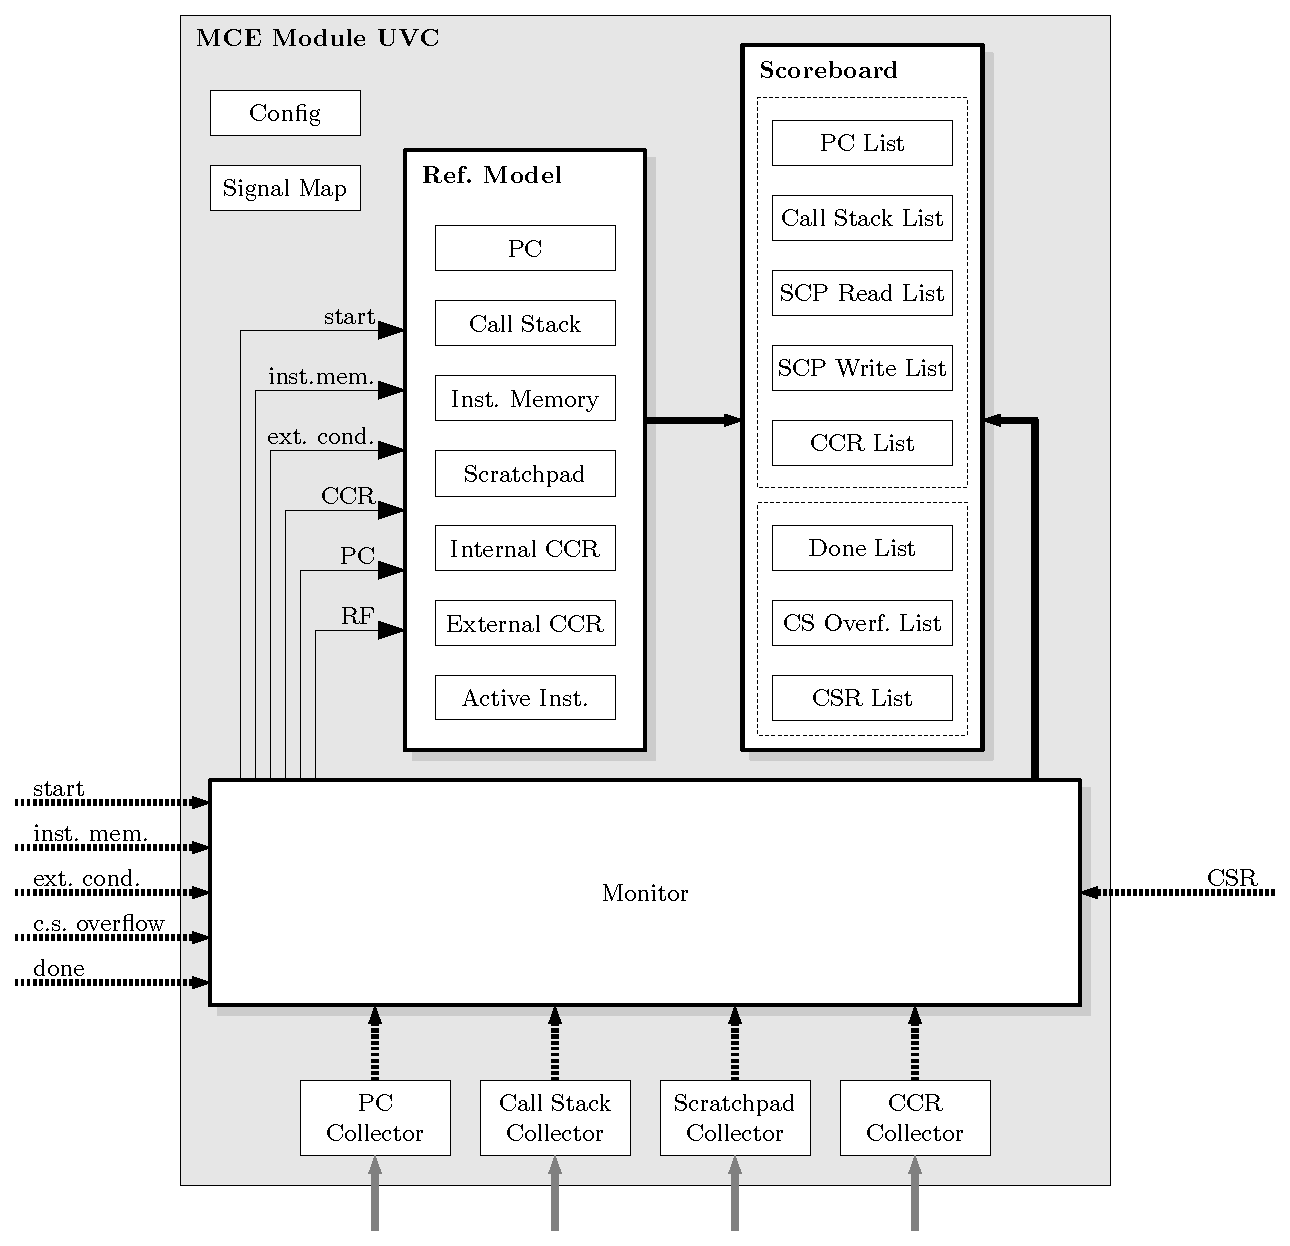
\includegraphics[scale=1.0]{images/mce_module_uvc}
 \caption{MCE Module UVC}
\label{fig:module_uvc}
\end{figure}

\subsubsection{Collectors}

Besides of the monitors of the interface UVCs, collectors are responsible for obtaining information about the DUT.
Where the monitors gather data from the interfaces of the design, the collectors receive their data from components inside of the MCE.
They are used to get a more precise insight on the current state of the DUT.
With these detailed information 
 

\paragraph{Program Counter Collector}

The program counter collector samples the current address of the PC.
It generates a new sequence item, whenever the PC is changed, while a program is running inside of the MCE.

\paragraph{Call Stack Collector}

The call stack collector observes the call stack of the design.
Whenever the index of the stack and therefore its size changes, a new transaction is created.
Thereby, a transaction contains the direction of the operation and the pushed or popped address, respectively.\\
In this process, the direction is derived from the change of the index.
If the index is incremented or an overflow occurs, a \emph{push} operation has been performed.
Whereas a decremented index indicates a \emph{pop} operation, except for an overflow.
Thereby, the exception of an call stack overflow occurs, if the call stack is currently empty and was full in the previous clock cycle.

\paragraph{Scratchpad Collector}

The scratchpad collector monitors the three ports of the scratchpad.
It generates sequence items for the read or write operations, respectively.
Thereby a sequence item contains the direction of the operation (read or write), the index of the port, the address of the accessed register as well as the read/written data.
Whereas the index of the write port is 0, of the first read port is 1 and of the second read port is 2.\\
When the normal program flow of the engine is disrupted by a conflicting external memory access, a single instruction can cause multiple consecutive write operations on the scratchpad. 
Since a memory access takes a unknown number of clock cycles to complete, it cannot be predicted, how many of these multiple write operations occur for an instruction.
However these multiple write operations do not change the state of the MCE.
Thus, it is sufficient to collect only the first operation of this series and ignore the following ones.
So no more than a single write operation is collected for a given instruction.\\
The MCE reads the scratchpad every clock cycle, while it is running a program.
Since reading the scratchpad does not influence its state, it is safe to do so.
Only the ALU determines, if the read data is required for the execution of an instruction.\\
Therefore the collector also takes the opcode of the instruction causing the read access into account.
So a transaction is only created, if the read access is really necessary for the execution of the instruction.

\paragraph{Condition Code Register Collector}

The condition code register collector observes the write port of the CCR.
Whenever a condition code is written into it, a new sequence item is created.
It consists of the index identifying a specific register of the CCR and the condition code, which is written.\\
Since the CCR does not contain a read port (each bit can be accessed directly), only the write port is monitored.

\subsubsection{Monitor}

The monitor is the central component of the module UVC.
It forwards the transactions received from the interface UVCs and the collectors to the remaining components of the module UVC.
All the communication between the monitor and the interface UVCs as well as the collectors is handled via TLM ports.
Thereby, the connected components can easily be exchanged on demand.\\
Additionally to handling the communication between components, the monitor also collects coverage.
This occurs, whenever the monitor receives a transaction from the collectors.

\subsubsection{Scoreboard}

The scoreboard is an important component for the self-checking testbench.
It verifies the proper operation of the DUT.
Therefor, it contains a list of transactions for the components, which determine the state of the design.
In figure~\ref{fig:scoreboard} it is displayed, which lists are included in the scoreboard.
These lists are grouped according to where their items are collected.
The lists of the \emph{design internal} group are used for the internal signals monitored by the collectors of the module UVC.
Furthermore the lists of the \emph{design interfaces} group contain data gathered from the interface UVCs.

\begin{figure}[htb]
 \centering
 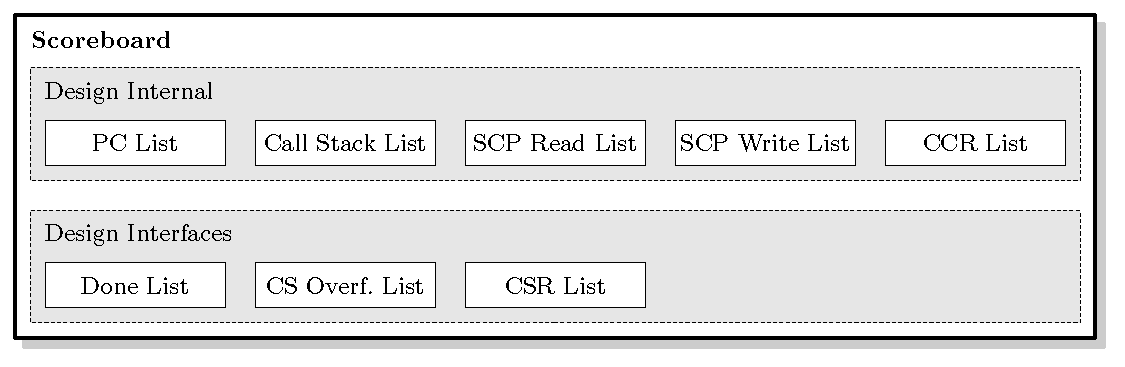
\includegraphics[width=1.0\textwidth,angle=0]{images/scoreboard}
 %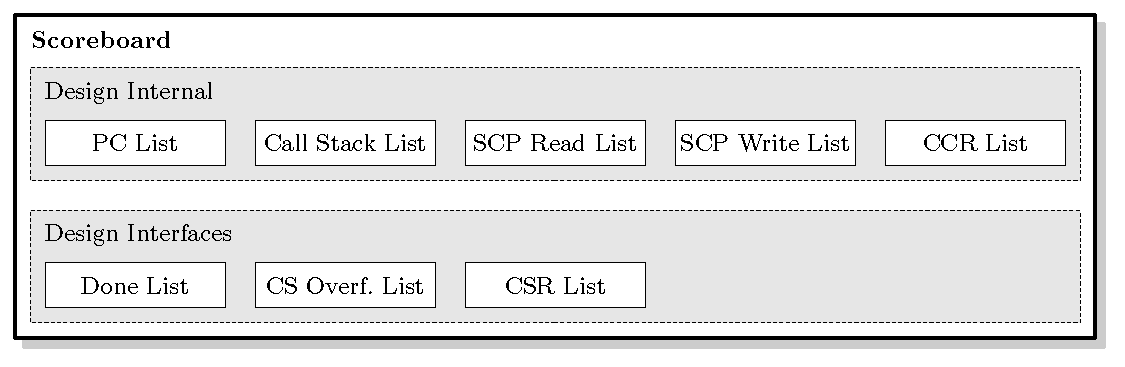
\includegraphics[scale=1.0]{images/scoreboard}
 \caption{Lists of the Scoreboard}
\label{fig:scoreboard}
\end{figure}

The procedure of checking within a general list is shown in figure~\ref{fig:scoreboard_flow}. 
Firstly, the predicted data from the reference model is added to the end of the list.
When a transaction is gathered by a collector or monitor of an interface UVC, it is send to the scoreboard.
After that, the received item is matched against the first item of the list.
If they match, both the reference model and the design produced equivalent data during their execution.
Otherwise either the testbench or the DUT contains a bug, which has to be fixed.\\
Needless to say, the list has to contain some items before any collected item can be matched.
Furthermore, at the end of a test run, all lists have to be empty.

\begin{figure}[htb]
 \centering
 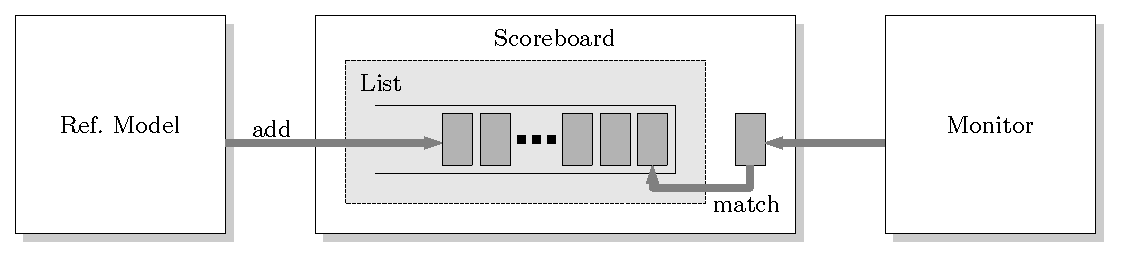
\includegraphics[width=1.0\textwidth,angle=0]{images/scoreboard_flow}
 %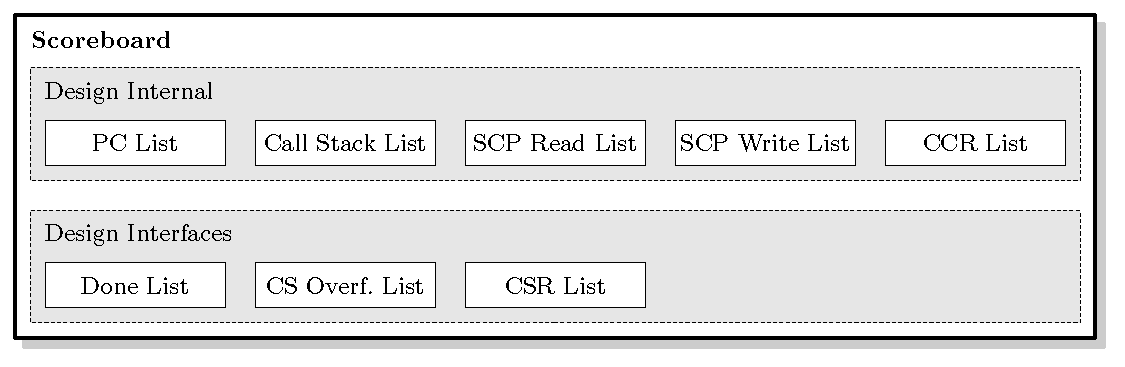
\includegraphics[scale=1.0]{images/scoreboard}
 \caption{Self-Checking within a General List}
\label{fig:scoreboard_flow}
\end{figure}

All lists except the scratchpad write list use this method.
Since the following instructions are executed while an external memory access is pending,
the order of the write operations on the scratchpad can change (see section~\ref{mem_access}).
However, the order of write operations on a specific register of the scratchpad is maintained.
Thus, collected scratchpad write operations are matched against the first item of the list with the same scratchpad address.
This is displayed in figure~\ref{fig:scoreboard_scp_write_flow}.

\begin{figure}[htb]
 \centering
 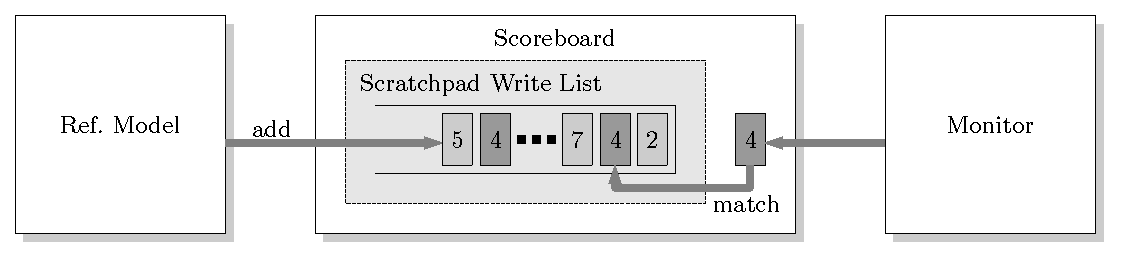
\includegraphics[width=1.0\textwidth,angle=0]{images/scoreboard_scp_write_flow}
 %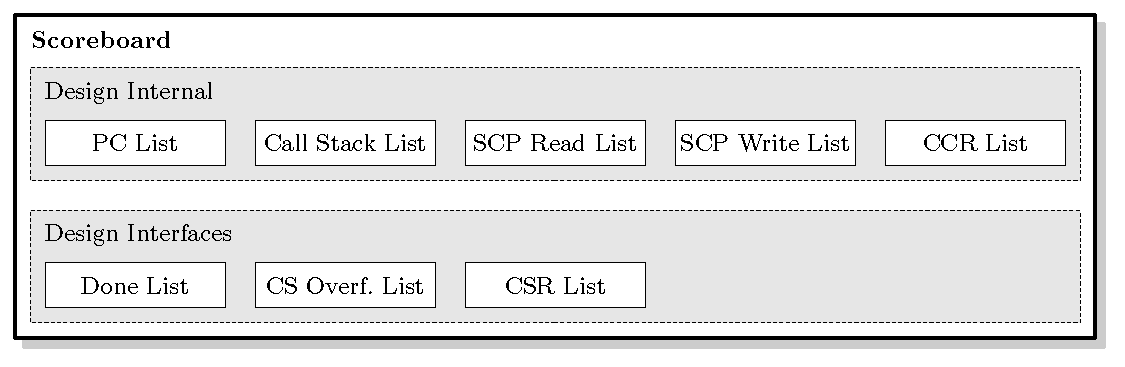
\includegraphics[scale=1.0]{images/scoreboard}
 \caption{Self-Checking within the Scratchpad Write List}
\label{fig:scoreboard_scp_write_flow}
\end{figure}


\subsubsection{Reference Model}

The reference model is a crucial part of the self-checking testbench. 
It predicts the behavior of the DUT for a given set of stimuli, which is then matched in the scoreboard against the transactions collected from the DUT.
The testbench of the MCE uses a reference model performing on the transaction level, since the self-checking of the testbench is performed on a functional level.
Following the architecture of the reference model is explained.

\paragraph{List of Active Instructions}

The central component of the reference model is the list of active instructions.
It contains all instructions, which already have been fetched from the instruction memory, but did not yet complete their execution.
This list is a queue with its last item being the instruction fetched at the earliest and its first item being the one fetched at the latest.
All operations of the reference model are performed on the items of this list.\\
An active instruction contains all information crucial to the execution of the instruction.
Its structure is shown in figure~\ref{fig:active_inst}.
Firstly it consists of the instruction itself and its address in the instruction memory.
Additionally the status indicating the current phase of execution of the active instruction within the reference model is hold.\\
Furthermore, data read or calculated during the execution of the operation are included.
These can be condition codes on the one hand or scratchpad data on the other hand.\\
The \emph{Guard Condition Code} is the condition code read from the CCR or the external condition code bits, which is used to decide, if a guarded instruction
or the BCC instruction is executed.
The \emph{CCR Write} condition code is produced by the ALU when the results of an instruction are calculated.\\
Data read from the scratchpad is stored in the \emph{Scratchpad Read} fields.
They can hold up to two items.
In the \emph{Scratchpad Write} field the result of an instruction is stored, which is written back to the scratchpad.\\
Not all types of instructions have to read or calculate all four types of data.
There is a \emph{valid} field available for each data item.
It indicates that the instructions has used or produced the related data field up to its current state of execution within the reference model.

\begin{figure}[htb]
 \centering
 %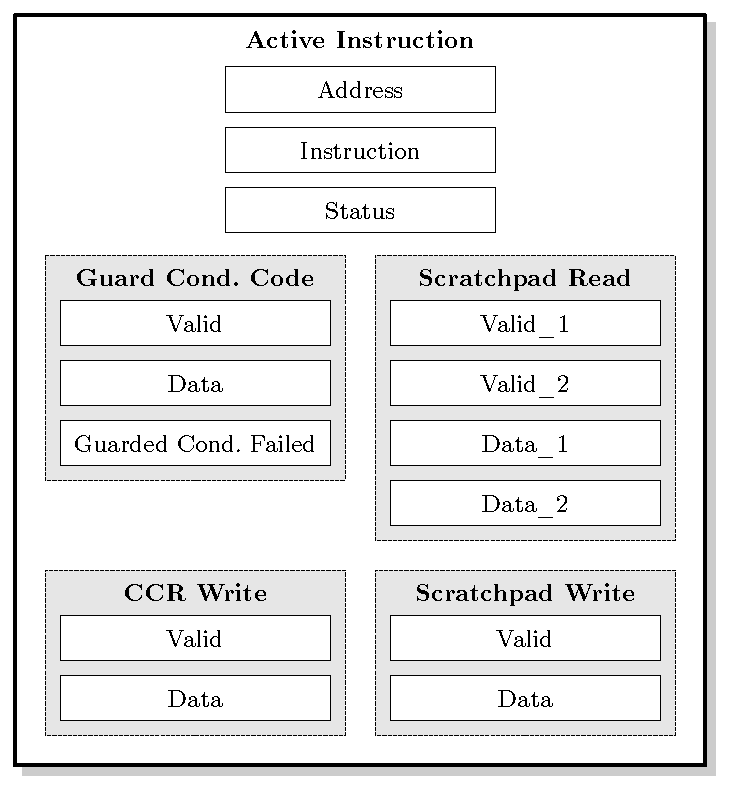
\includegraphics[width=1.0\textwidth,angle=0]{images/active_inst}
 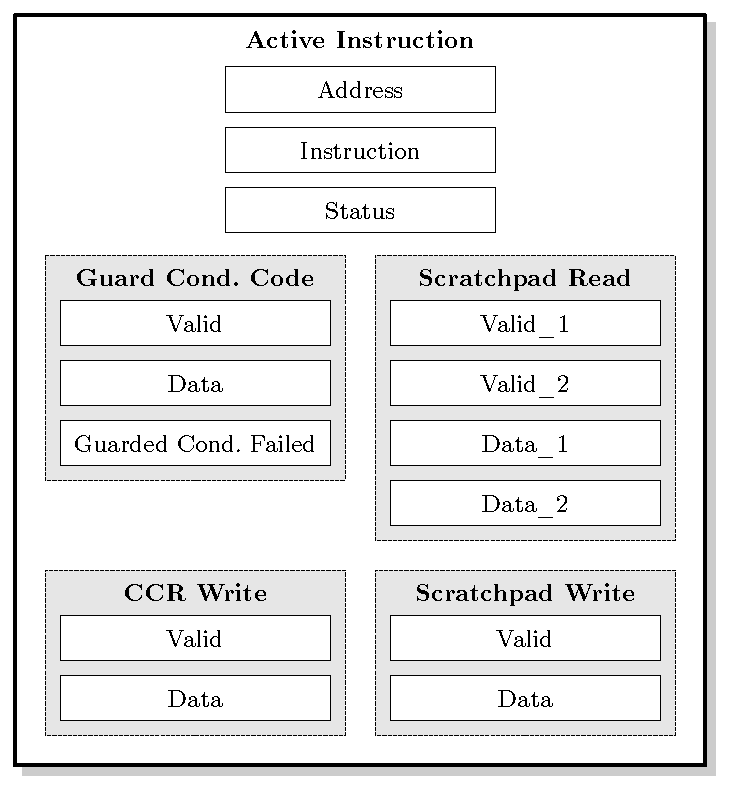
\includegraphics[scale=1.0]{images/active_inst}
 \caption{Structure of an Active Instruction}
\label{fig:active_inst}
\end{figure}

\paragraph{Instruction Execution Flow}

The execution of an instruction in the reference model is divided into multiple phases.
Thereby, the current state of an active instruction is indicated by its status field.
The available states are shown in figure~\ref{fig:ref_model_phases}.
It displays the finite state machine (FSM) each instruction passes through.
The opcode of the instruction determines, which states of the FSM are traversed by the instruction, when it is executed.
Thereby each instruction tries to pass through the FSM as far as possible.
It either reaches the acceptor state \emph{complete}, which indicates that the instruction has finished its execution, or its execution is interrupted by a
conflict (see section~\ref{stall_barrier}).\\
A new instruction is always fetched, whenever the PC collector sends a sequence item to the monitor.
This indicates, that the MCE has updated its internal PC value.
After that, each instruction tries to move on within the FSM as far as possible.
The list of active instructions is thereby traversed starting with the oldest instruction down to the newest fetched one.
This ensures the in-order execution of the instructions.\\
Since the MCE uses data-forwarding to hide the delays between reading and writing the scratchpad, it can be ignored, that both events occur in different
pipeline stages of the engine.
This simplifies the FSM of the reference model.
Only reading from the external CSR and writing to the CCR require special handling.
That is because the delay of the pipeline stages is not hidden for these operations.\\
Following, the operations performed within each state of the FSM are presented in more detail.

\begin{figure}[htb]
 \centering
 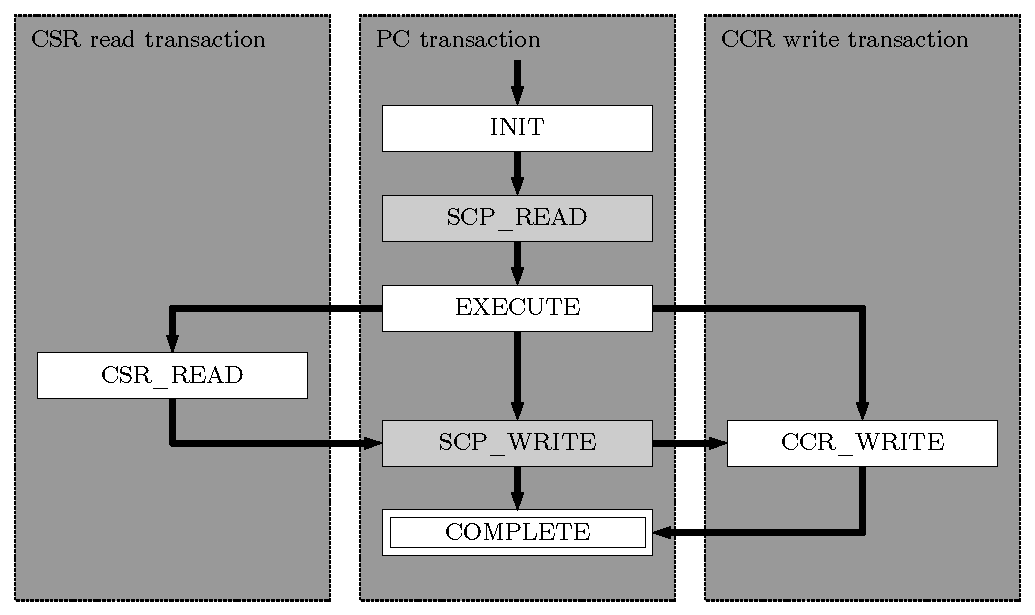
\includegraphics[width=1.0\textwidth,angle=0]{images/ref_model_phases}
 %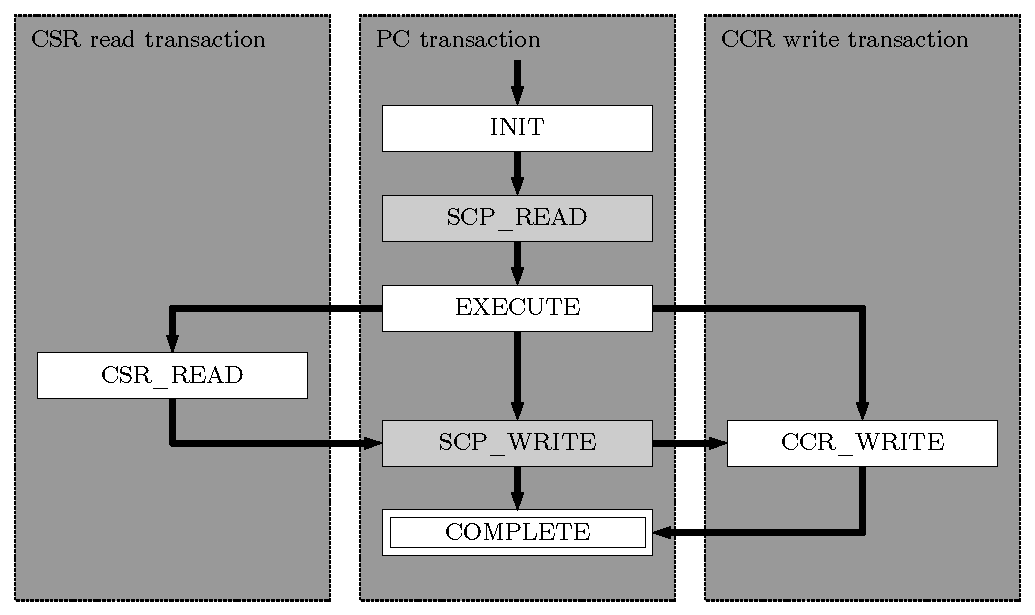
\includegraphics[scale=1.0]{images/ref_model_phases}
 \caption{State Machine of the Instruction Execution Flow}
\label{fig:ref_model_phases}
\end{figure}

\subparagraph{INIT State}

After an instruction has been fetched, it starts in the \emph{INIT} state.
Here it is determined, if a conditional instruction (GARITH, GLOGIC or BCC) is executed at all.
If the conditional execution fails, the instruction still traverses the whole FSM, but does not perform any operations inside of a state.
By that, the order of the instructions is maintained.\\
Additionally the next PC is calculated by either jumping to the address included in the CFLOW instruction or by incrementing it for other types of instructions
with the exception of the STOP instruction, which does not generate a new PC value.
If a new PC value has been calculated, it is also added to its corresponding list in the scoreboard.
By that, the predicted PC value is always added to the scoreboard before the one collected from the DUT is matched against it.
Furthermore , if the STOP instruction is executed, an item is added to the \emph{done} list of the scoreboard.
Finally, the \emph{INIT} phase is completed and the instruction moves on to the next state.

\subparagraph{SCP\_READ State}

In the \emph{SCP\_READ} state it is checked, if reading from the scratchpad would result in a conflict with a previously scheduled instruction, which has not
already completed its execution (see section~\ref{stall_barrier}).
If no conflict occurs, the required registers of the scratchpad are read.
Their addresses are indicated by the instruction resulting in four possible behaviors.
Firstly, the instruction does not need any data from the scratchpad, so no data is read.
Secondly, the instruction performs its operation on its destination register.
Then the data is read from the scratchpad address identified by the \emph{RD} field of the instruction.
Furthermore, the instruction does only require a single operand, so only the register of the scratchpad is read, which is determined by the \emph{RS1} field of
the instruction.
Finally, the instruction needs two operands.
Then both values are read from the scratchpad using the \emph{RS1} and \emph{RS2} fields of the instruction.\\
Whenever data is read from the scratchpad of the reference model, an item is added to the scratchpad read list of the scoreboard.
Each item contains the predicted values of a single read operation and the corresponding address of the scratchpad register.
So considering the four behaviors mentioned above, an instruction can add up to two items to the scratchpad read list of the scoreboard.
When two items are added for a single instruction, the item reading the scratchpad register identified by the \emph{RS1} field of the instruction is
added first.
Corresponding, the sequence item collected from the first read port of the scratchpad within the DUT has to be matched firstly for these instructions.
After that, the \emph{SCP\_READ} phase is finished and the active instruction moves on to the next state of the FSM.

\subparagraph{EXECUTE State}

In the \emph{EXECUTE} state the operation of the instruction is performed.
The exact operation is thereby determined by the opcode of the instruction.
Instructions of the CFLOW group do not perform any operations in this phase.
The other instructions predict the operations of the ALU within the DUT (except LDR and STR instructions).
Thereby the required operands are the values read from the scratchpad in the previous state of the FSM or immediate values directly included in the instruction
itself.
The results are cached within the active instruction for further use in the next states of the FSM.\\
For the LDR and STR instructions transactions are generated, that are added to the CSR list of the scoreboard.
They contain the calculated address of the accessed register within the CSR as well as a field identifying the direction of the operation (READ or WRITE).
The data written into the CSR is also included for the STR instruction.\\
The next state of the active instruction is dependent on its opcode.
Thereby the LDR instruction is the only one proceeding to the \emph{CSR\_READ} State, since its result cannot be determined immediately.
The other instructions write their results into the scratchpad or CCR.
Instructions, which only produced data for the CCR, move on to the \emph{CCR\_WRITE} state.
All other instructions continue to the \emph{SCP\_WRITE} state.

\subparagraph{SCP\_WRITE State}

In the \emph{SCP\_WRITE} state it is checked, if writing to the scratchpad would result in a conflict with a pending LDR instruction accessing the external
memory (see section~\ref{stall_barrier}).
If no conflict occurs, the result of the execution of the instruction is written into the scratchpad.
The exact register of the scratchpad is thereby identified by the \emph{RD} field of the instruction.
When the predicted result is written into the scratchpad of the reference model, an item is added to the scratchpad write list of the scoreboard.
It contains the predicted result and the address of the register , which is written.
If an active instruction does not contain any results, which have to be written back into the scratchpad, no operation is performed in the \emph{SCP\_WRITE}
phase.
The next state of the instruction depends on its opcode.
Thereby, active instruction containing also results for the CCR proceed to the \emph{CCR\_WRITE} state.
All other instructions continue to the \emph{COMPLETE} state.

\subparagraph{COMPLETE State}

The \emph{COMPLETE} state indicates, that an active instruction has been executed successfully.
No operations are performed within this state.
It is used to mark active instructions, which can be removed from the list of active instructions.

\subparagraph{CCR\_WRITE State}

Instructions, that reach the \emph{CCR\_WRITE} state, are not updated like the other states, when a PC transaction arrives from the PC collector.
They are only updated, when a CCR write transaction is received from the CCR collector.
Thereby only the oldest instruction in the \emph{CCR\_WRITE} state is updated.
So each instruction in this state needs an individual CCR write transaction to proceed its flow within the FSM.\\
The reference model is thereby independent of the actual amount of clock cycles between fetching an instruction and writing its result into the CCR.
It is only important, that the separate resulting condition codes are written into the CCR in order and the resulting behavior of the following instructions is
correct.\\
This leads to a more general reference model, that is completely independent of the amount of pipeline stages used within the MCE.
This reduces the risk of having to adjust the reference model, when the DUT is changed.
Nevertheless, it has to be checked, that the delay is constant for a specific implementation of the MCE.
Therefor a separate \emph{SystemVerilog Assertion} (SVA) is used to verify, that each CCR write occurs three clock cycles after the causing instruction has been
fetched.\\
When the update of an active instruction in the \emph{CCR\_WRITE} state is triggered, an item is added to the CCR write list of the scoreboard.
This sequence item contains the address specifying the register of the CCR given by the \emph{crs} field of the instruction, as well as the predicted resulting
condition code.
It is important, that the update of the reference model is triggered before the collected item is matched in the scoreboard, since the predicted item has to be
added to the list before the collected one can be matched against it.\\
As writing the resulting condition code into the CCR is always the last operation of an instruction, each active instruction can go on to the \emph{COMPLETE}
state.

\subparagraph{CSR\_READ State}

Since reading from the external CSR is the only operation, which needs a variable amount of clock cycles to complete, it is handled separately from the other
operations.
It moves to the \emph{CSR\_READ} state after the \emph{EXECUTE} state, while waiting for the CSR read access to complete.
A completed read access on the external memory is indicated by an read transaction received from the CSR interface UVC.
It is generated and sent to the module UVC whenever the monitor of the CSR interface UVC samples an active \emph{access\_complete} signal after \emph{read\_en}
has been asserted.\\
Similar to an instruction in the \emph{CCR\_WRITE} state, a received transaction only moves the oldest instruction in the \emph{CSR\_READ}
state on to the next state. So each instruction in the \emph{CSR\_READ} state requires a separate transaction. 
When such a transaction is received, the read data is extracted from the sequence item and cached in the active instruction as its result.
After that the instruction goes on to the \emph{SCP\_WRITE} state to write its result back into the scratchpad.

\paragraph{Stall Barrier}\label{stall_barrier}

When the MCE initiates an operation on the CSR, it can take multiple clock cycles until the request is completed.
Instead of being stalled for this period, the engine continues to execute the it following instructions.
The MCE only stalls its execution, when a conflict occurs between the pending external memory access and one of the it following instructions.\\
So the reference model also has to continue the execution of instructions, while a CSR access is pending.
But it has to ensure, that its internal states remain equivalent to the ones of a unit, that executes instructions strictly in order.
Since the scratchpad is the only internal memory, that is manipulated by a CSR access, it has to be guaranteed, that the destination register of the pending CSR
access is not manipulated by one of the it following instructions.\\
To achieve this, the stall barrier is used in the reference model. It prevents active instructions from accessing the destination register of a pending CSR
access. Furthermore, it ensures that all instructions are executed in order and do not pass each other.
The FSM of the reference model cannot be stalled completely, as soon as a conflict occurs, since transactions are still collected from other pipeline stages of
the MCE.
So the predicted items have to be added to the scoreboard before these transactions are collected.
When a conflict occurs between a pending LDR instruction and one of the it following instructions, the stall barrier is set to the specific state,
where the conflict occurs.
This state can either be \emph{SCP\_READ} or \emph{SCP\_WRITE}.\\
It prevents all instructions from performing operations within the state specified by the stall barrier or other states following this state.
On the one hand, this prevents instructions from accessing the destination register of the pending LDR instruction and on the other hand, it prevents
instructions from passing each other.\\
The stall barrier is set to \emph{SCP\_WRITE}, if an instruction wants to write its results into the same register of the scratchpad as the pending LDR
instruction.
Corresponding, the stall barrier is set to \emph{SCP\_READ}, if an instruction wants to read from the destination register of a pending LDR instruction.
Furthermore, the stall barrier is also set to \emph{SCP\_READ}, if an instruction wants to read from the destination register of an instruction with a pending
write operation on the scratchpad. This can only occur, has already been set to \emph{SCP\_WRITE}.
When the reference model receives a read transaction from the CSR interface UVC, the stall barrier is reset to the acceptor state \emph{COMPLETE}.\\
Since the sequence item for a STR instruction can already be added to the CSR list of the scoreboard within the \emph{EXECUTE} state, the reference model does
not have to wait for the external memory access to be completed.
Therefore, the reference model does not have to be stalled for this operation, in contrary to the MCE itself.

\begin{figure}[htb]
 \centering
 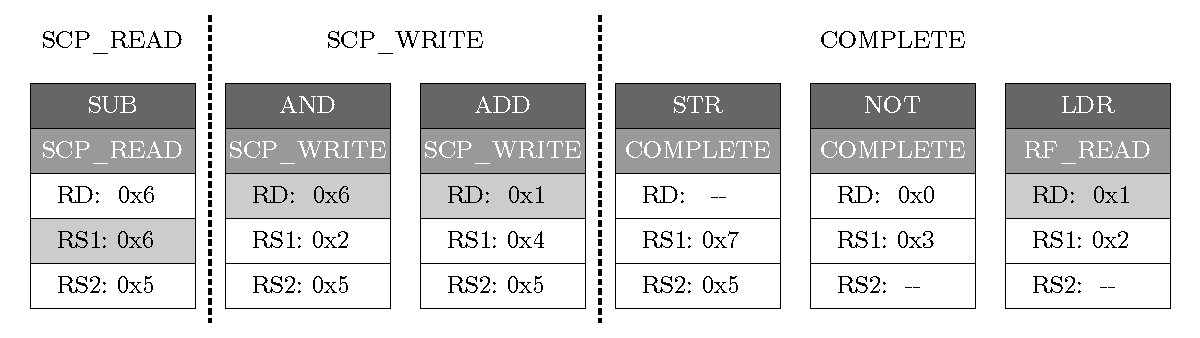
\includegraphics[width=1.0\textwidth,angle=0]{images/stall_barrier_example}
 %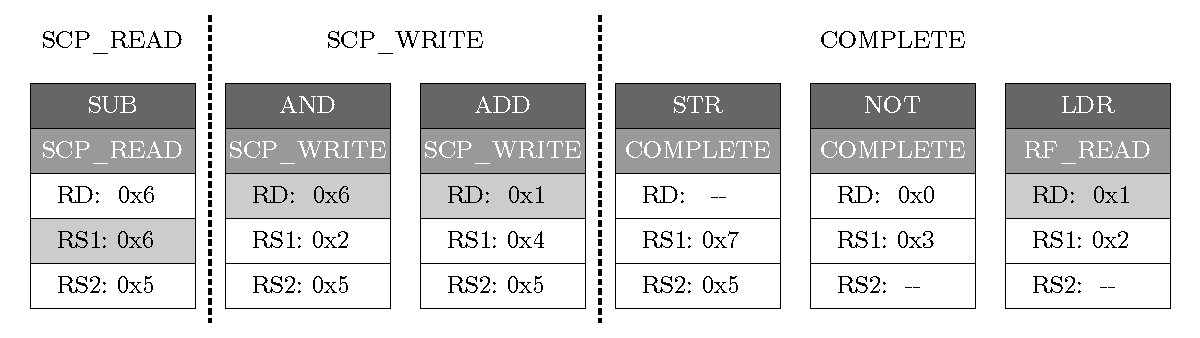
\includegraphics[scale=1.0]{images/stall_barrier_example}
 \caption{Example of the Stall Barrier}
\label{fig:stall_barrier_example}
\end{figure}

An example of the behavior of the stall barrier is shown in figure~\ref{fig:stall_barrier_example}.
The reference model is still waiting for the LDR instruction to be completed (indicated by the \emph{RF\_READ} state).
This means, that register \emph{0x1} of the scratchpad is the critical one, since it is the destination of the CSR read operation.
As the it following NOT and STR instructions do not access this register, the stall barrier does remain at the acceptor state and both instructions can be
completed.
The ADD instruction also wants to write the same register as the pending LDR instruction.
This sets the stall barrier to \emph{SCP\_WRITE} and prevents the ADD instruction and all following ones from writing into the scratchpad.
The AND instruction can only reach the \emph{SCP\_WRITE} state, due to the stall barrier.
Finally, the SUB instruction wants to read register 0x6, but this register is the destination of a pending write operation (AND instruction).
Therefore, the stall barrier is set to \emph{SCP\_READ}, preventing this read operation.

\paragraph{Removing Completed Instructions}

Completed instructions have to be removed from the list of active instructions.
They are removed in order from the list, since removing an instructions, also prints its content to the console.
This means, that a completed instruction is not yet removed, if a previous instruction has not completed its execution.
Through that, the completed STR and NOT instructions of figure~\ref{fig:stall_barrier_example} still remain in the list, until the LDR instruction has also
reached the \emph{COMPLETE} state.\\
Most important is, that coverage is collected for the instruction, whenever a completed instruction is removed from the list of active instructions.

\subsection{Virtual Sequence Driver}

During the verification the execution of a program within the DUT is controlled by the testbench.
The individual interfaces of the MCE are thereby controlled by the connected agents.
Since a test needs to coordinate all these agents at once, a virtual sequence driver is used to direct the individual parts of a test to the corresponding
sequence drivers within the agents. The interaction between these components is displayed in figure~\ref{fig:vsd}.

\begin{figure}[htb]
 \centering
 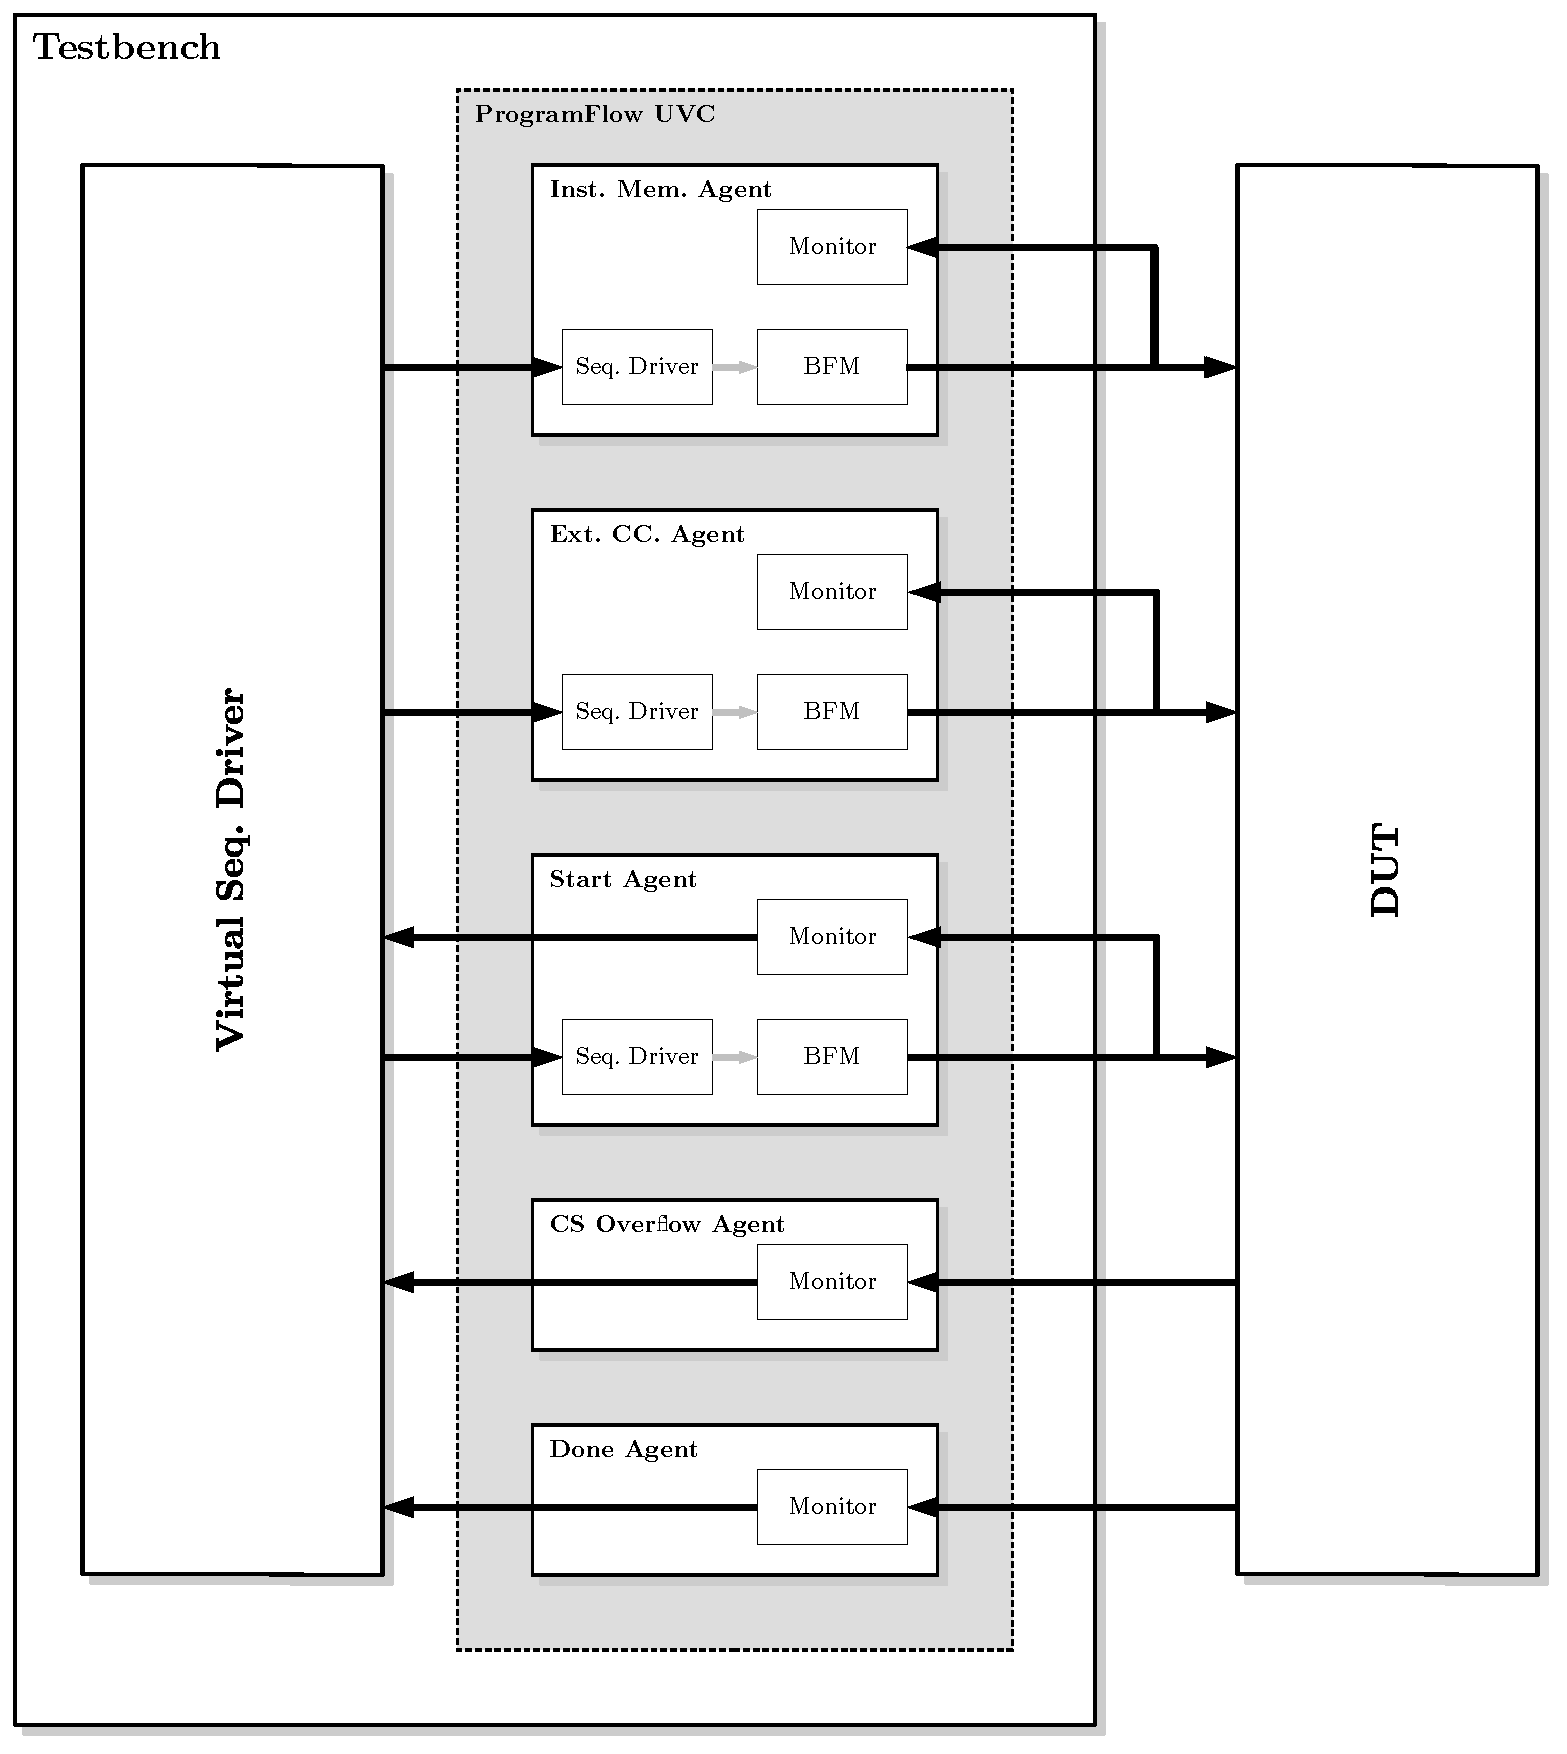
\includegraphics[width=0.9\textwidth,angle=0]{images/vsd}
 %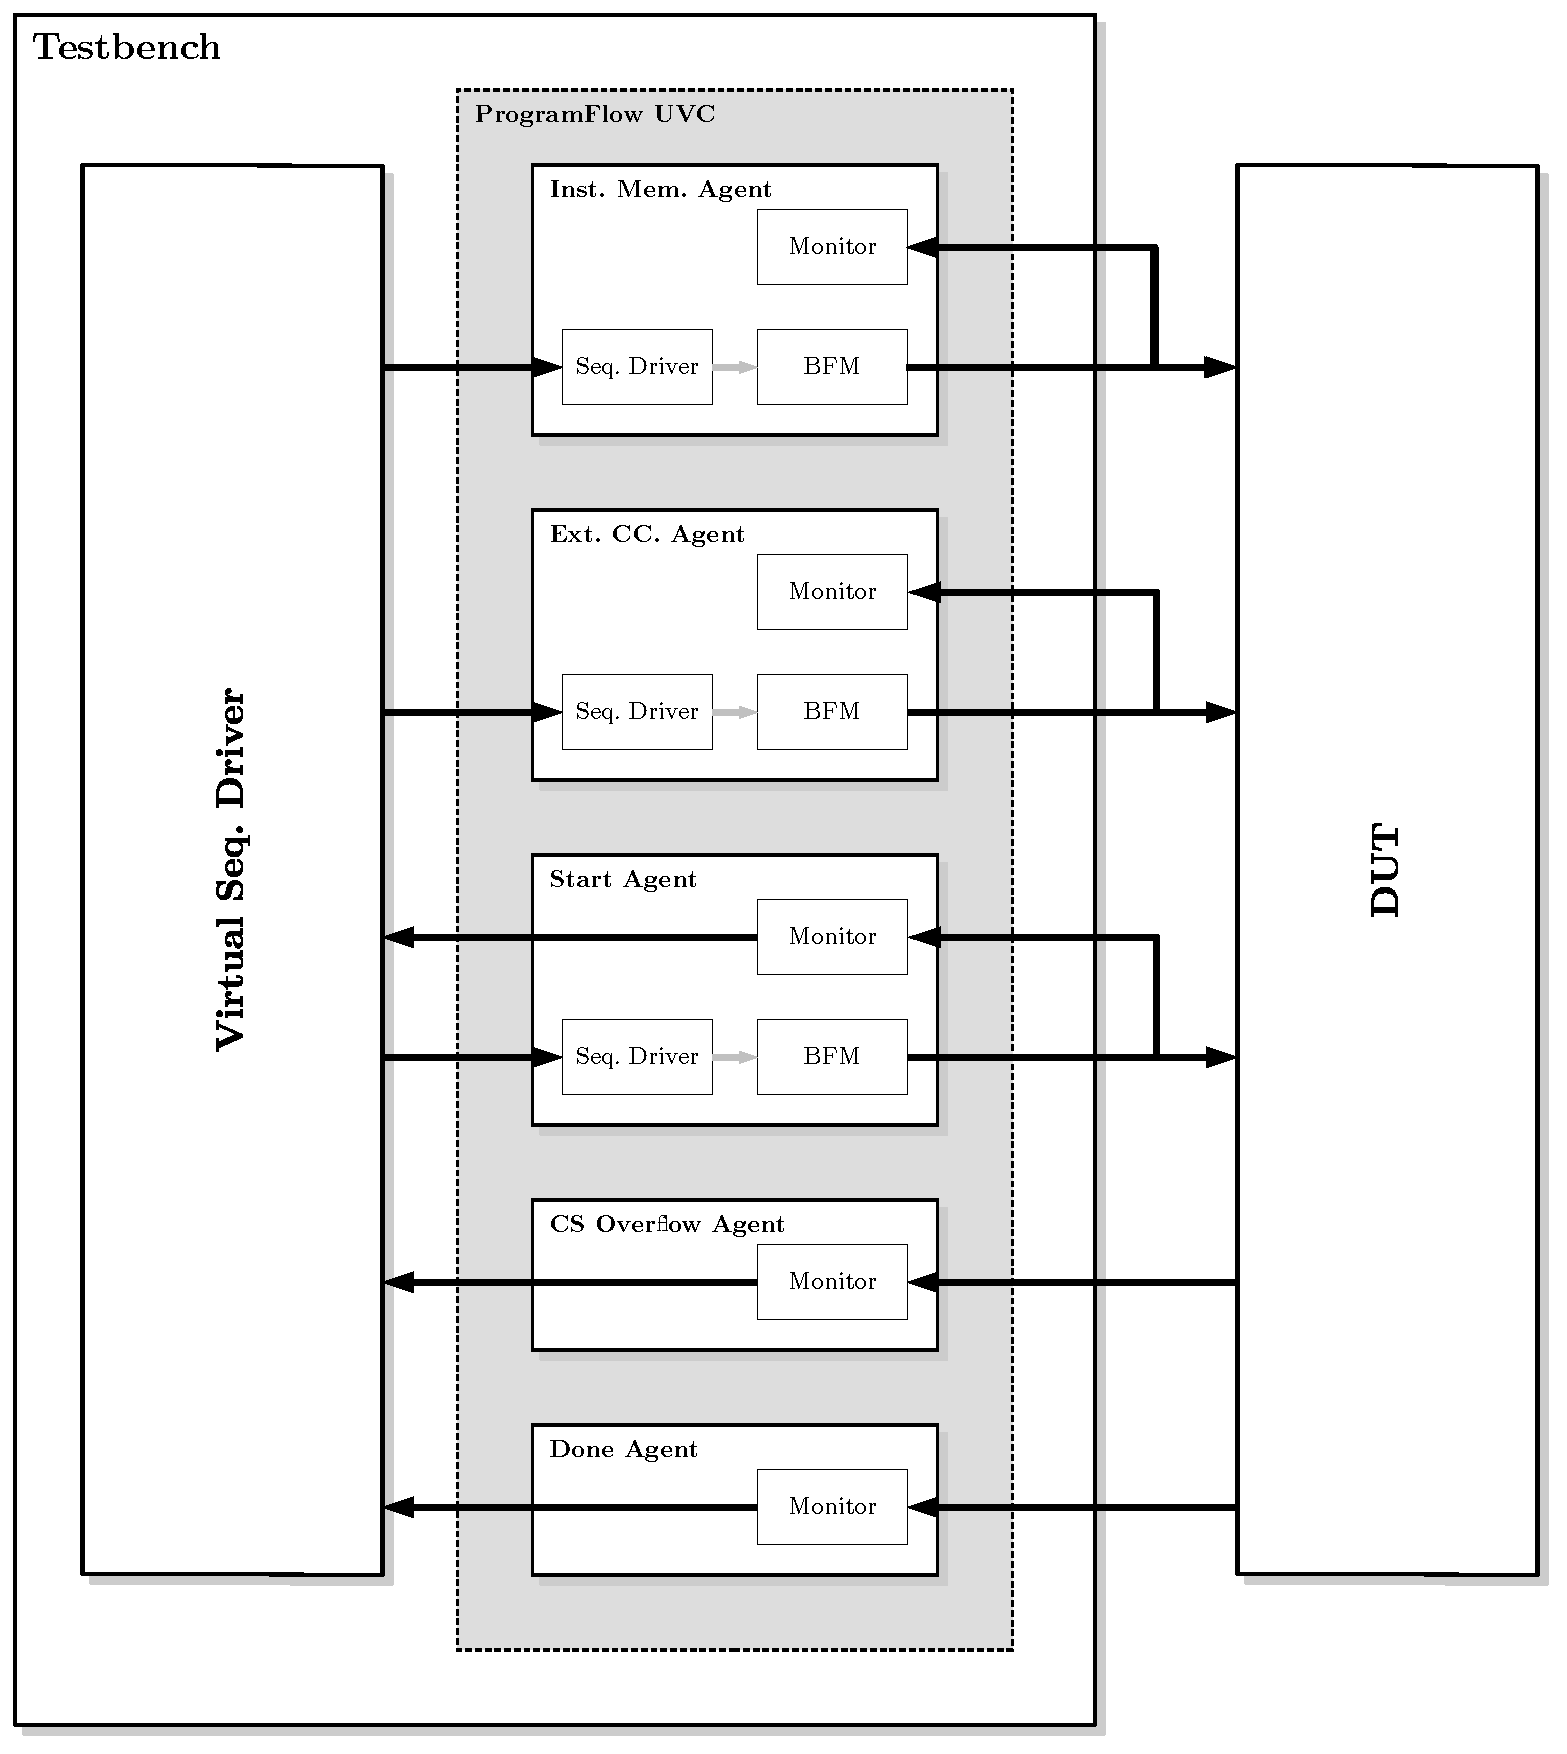
\includegraphics[scale=1.0]{images/vsd}
 \caption{Interaction Between the Virtual Sequence Driver and the Agents of the ProgramFlow UVC}
\label{fig:vsd}
\end{figure}

The virtual sequence driver signs the sequence driver of the instruction memory agent to write the instructions building the program into the instruction memory
of the MCE.
Additionally the external condition code bits can be asserted via the sequence driver of the corresponding agent.
After that, the execution of the program is started via the sequence driver of the start agent.\\
Since the virtual sequence driver does not know, when the execution of a program is stopped, without additional information, it has to be informed about the
execution status of a program.
So the monitor of the start agent informs it about the start of a program and the monitors of the call stack overflow and done agents about its end.
This ensures on the one hand, that a test is not quit before a program has completed its execution within the DUT and on the other hand enables the test to
start another program after the first one completed.\\
The CSR interface UVC contains a slave agent, which automatically responds to access on the external memory.
Therefore its sequence driver does not have to be controlled by the virtual sequence driver.

\subsection{Test Library}

Tests are used to generate the stimuli for the interfaces of the DUT. They write the instructions into the instruction memory, assert external condition code
bits and start the execution of the program within the MCE. Multiple tests are used to generate various kinds of inputs, depending on the major functionalities,
which are tested. Thereby the test are shaped mostly in  a general manner, so each test can cover as much functionality of the MCE as possible. Each test can
then be run with different seeds, resulting in different input patterns within the boundaries of the test \cite{sv_verification}.
Following are the different kinds of tests explained, which are used within the testbench.

\subsubsection{Simple Test}

The simple test initiates the scratchpad using a single LDI instruction for each scratchpad address. 
Followed by a STOP instruction to end the program.
It is used to see as quickly as possible, if the testbench has been setup correctly.
Therefore, it is kept short to receive the results in a couple of seconds.
A single run of the other more complex tests can take up to multiple minutes to complete.

\subsubsection{Non-Branching Test}

The non-branching test is used to cover the functionalities of the ALU as well as the memory interface.
In combination with that, it also covers the access on the scratchpad and CCR.
It uses multiple interfaces of the MCE including the instruction memory interface, start interface, done interface and CSR interface.
The main objective is thereby to execute a single program using multiple non-branching instructions.
Meaning, that it only executes instructions, which are not included in the CFLOW group.
The opcode of the instructions as well as the remaining fields are thereby randomly generated, so a variety of combinations of different instructions is
executed.
The structure of the non-branching test is shown in figure~\ref{fig:non_branching_test}.

\begin{figure}[htb]
 \centering
 %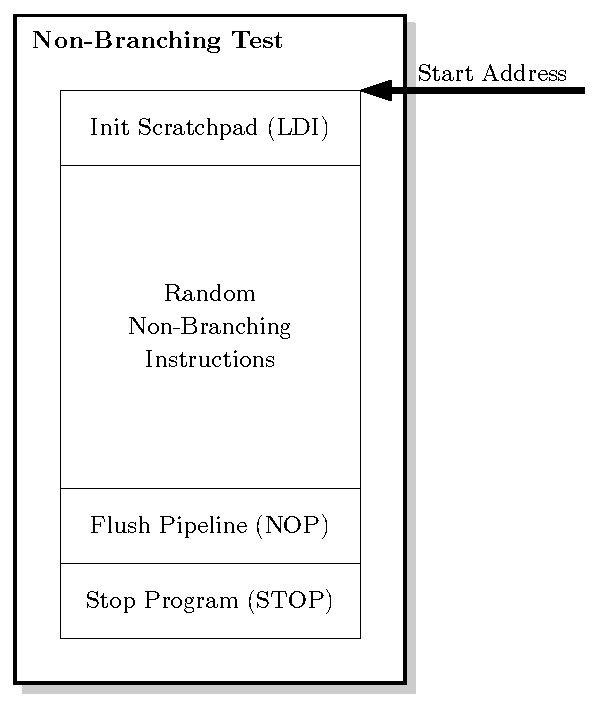
\includegraphics[width=1.0\textwidth,angle=0]{images/non_branching_test}
 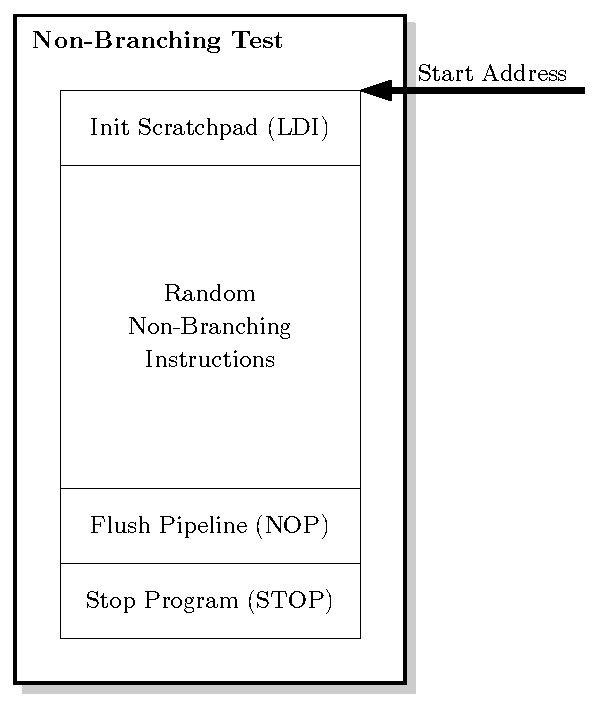
\includegraphics[scale=1.0]{images/non_branching_test}
 \caption{Structure of the Non-Branching Test}
\label{fig:non_branching_test}
\end{figure}

The start address of the program is chosen randomly from the address space of the instruction memory.
To ensure, that no read operation is performed on an uninitialized register of the scratchpad, each register is firstly initialized using the LDI instruction.
After that, a random amount of non-branching instructions is written into the instruction memory.
At the end, a couple of NOP instructions is written, to flush the pipeline of the MCE and thereby ensure, that all previous operations have completed.
Finally a single STOP instruction is written to stop the program.
After all instructions are written into the instruction memory, the program is started.



\subsubsection{Branching Test}

The structure of the branching test is similar to the one of the non-branching test. The start address is selected randomly, first the scratchpad is initialized
with LDI instructions and at the end the pipeline of the MCE is flushed with NOP instructions followed by a single STOP instruction to end the program.
The difference is, that the branching test also includes the instructions of the CFLOW group into its set of random instructions.
Since with purely random instructions the program could end in a infinity loop, some rules have to ensure, that the program always terminates.\\
Each branching within the program is structured like a function call. Meaning, that the program jumps to a specific address, executes an amount of instructions
and then returns to the calling instruction.
The CFLOW group contains three branching instruction (CALL, JMP, BCC). Since the CALL instruction is designated for function calls, its usage is the simplest.
Whenever a CALL instruction is executed, the address of the following instruction is pushed to the call stack. So the RET function just has to be called at the
end of the sub-program. Through that, the PC is automatically restored.\\

\begin{figure}[htb]
 \centering
 %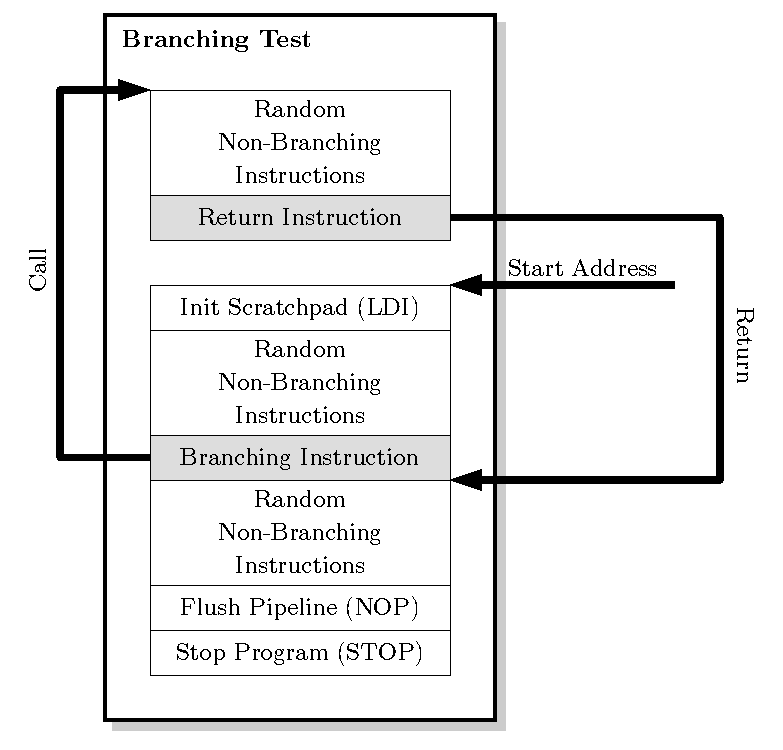
\includegraphics[width=1.0\textwidth,angle=0]{images/branching_test}
 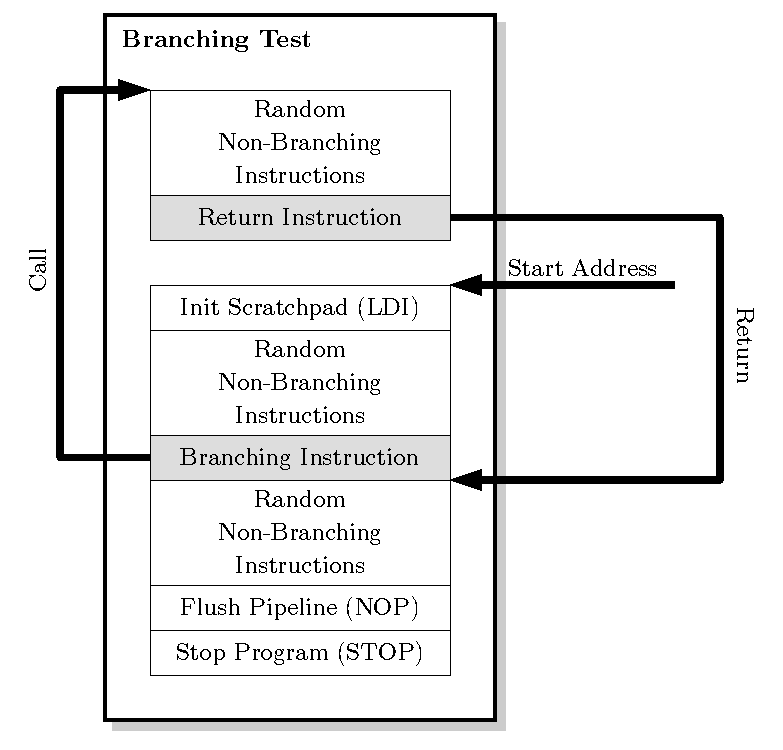
\includegraphics[scale=1.0]{images/branching_test}
 \caption{Structure of the Branching Test}
\label{fig:branching_test}
\end{figure}

Since the addresses of the next instructions are not stored for JMP and BCC instructions, this has to be done within the test itself.
Thus, the return address is stored within the test and instead of the RET instruction a JMP instruction is used to restore the PC to the return address.\\
These three types of function calls can also be nested within each other. 
So on the one hand this test checks, that the PC is always set to the right value and on the other hand verifies the whole call stack.
In addition to the STOP instruction at the end of the program, the branching test can also end, when a call stack overflow occurs.
Since each function call requires additional address space within the instruction memory, it can occur, that the memory is full.
In this case only non-branching instructions are generated to fill the already allocated address space.
The STOP instruction is the only one, that is not allowed to occur randomly within the test.\\
The structure of the branching test with a single function call is shown in figure~\ref{fig:branching_test}.



\subsubsection{Multi-Start Branching and Non-Branching Test}

To verify the behavior of the MCE  for all combinations of instructions, a version the branching and non-branching test is available, that also supports the
STOP instruction in its set of random instructions. For instructions other than the STOP instruction, the behavior of both tests is equivalent to the ones not
supporting the STOP instruction.\\
The multi-start versions also contain a list of start addresses. 
Whenever a STOP instruction is generated, the address of the it following instruction is added to the list of start instructions.
So each time the execution of the MCE is stopped via a STOP instruction, it can be restarted by popping the next start address from the list.
Since the test cannot know by itself, when the execution is interrupted, the monitor of the done agent informs the test, that the done signal has been asserted.
By that, the test can directly restart with the next instruction.

\subsubsection{External Condition Code Test}

The external condition code test is a version of the branching test, which also supports controlling the external condition code bits agent.
Prior to starting the execution of the program, the external condition code bits can be set. 
Since only the BCC instruction makes use of the external condition code bits, a non-branching test supporting external condition code bits is not required.
